\section{Abstract}
Assigned: David Demasi \cite{brandon:2008}

\subsection{Header}
\begin{description}
\item[Principal Investigator] Hamid Ossareh
\item[University] University of Vermont and Vermont Technical College
\end{description}

\subsection{Problem Description}
For this mission, the three CubeSats, which are initially separated
from one another in radial velocities by $0.1 m/s$, will autonomously
and optimally fire their thrusters to get into an intermediate
triangular formation after $\frac{1}{3}$ of an orbital period (1861
seconds), and then fire their thrusters again to get into a final
linear formation after one full orbital period (5582 seconds).

This is achieved by solving an optimization problem on-board the
CubeSat computers. The optimization problem is a mixed-integer linear
program, and calculates the thruster timing, duration, and magnitude
to achieve collision-free formation with minimum fuel usage. In the
optimization problem, we assume that all three satellites start from
the same initial positions (origin in local vertical local horizontal
or LVLH frame), make an intermediate triangular formation, and end up
on a linear formation where they are spatially separated about $478.8m$
(calculated from data available to us) from one another after one
orbital period in along-track direction.

For the calculations and figures that follow, we assumed the following
orbital parameters for the initial center of mass of the three
satellites, but these parameters can be adapted to any circular low
earth orbit:

\begin{itemize}
  \item semi major axis $a = 6800 Km$
  \item Eccentricity $e = 0$
  \item Right ascension of the ascending node $(RAAN):-0.01675^{\circ}$
  \item Geodesic latitude $\omega = 0^{\circ}$
  \item True anomaly $v = 0^{\circ}$
  \item Inclination angle $i = 25^{\circ}$
\end{itemize}

The optimization problem uses the linearized J2-perturbed dynamics,
which are shown to be accurate in the timescales under consideration
for circular orbits. We assume our thruster capability is within:

\[[-10, 10] mN\]

These optimal control and maneuvers are obtained as a solution to a
trajectory optimization (TO) problem, formulated as a mixed-integer
linear program, given below. This TO problem has two parts – in the
first part we obtain fuel optimal trajectories, controls and
assignments to move from the origin to a ``triangular formation'' in
LVLH frame and from the second part we find optimal trajectories,
controls and assignments as the satellites move from the triangular
formation to a final linear formation. For simplicity, we provide here
the basic structure of the minimum fuel TO algorithm, which is
replicated twice for different $t_f$'s (for example $T/3$ in the first
case and $2T/3$ in the second) and different final points (for
example, vertices of the triangular formation in the first case, three
equidistant points on a straight line for the second case).

$min J_{|u,x|} = \sum_{i=1}^{N} \sum_{p=0}^{Q-1} \sum_{k=1}^{v} | u_{ik} (P)|$
subject to
\begin{itemize}
\item State space constraints:
  $x_i(p+1) = Ax_i(p)+Bu_i(p)$ with $i = 1,2,...,N$ and $p = 0,1,2,...,T-1$,
\item initial state $x_i(0) = x_{iS}$,
\item final configuration constraint
  $x_{iT} = \sum_{j=1}^{N}b_{ij}x_{jD}$
  with $\sum_{i=1}^{N}b_{ij} = \sum_{j=1}^{N}b_{ij} = 1$,
  where $b_{ij}$
  is a binary variable and responsible for deciding the assignment of
  each of these final positions to a satellite,
\item actuator saturation constraint $u_{k,max} \leq u_{ik}(p) \leq u_{k,max}$.
\end{itemize}

Figure \ref{fig:trajectories} presents the trajectories of the three
satellites undergoing aforementioned maneuvers along the way. Starting
point is marked with ``x'', intermediate triangle formation is shown
with red and all three terminal points are marked with squares in
respective colors. All axes represent the satellite coordinates in the
LVLH frame relative to the target orbit defined by the above orbital
parameters.

\begin{figure}
\centering

\begin{subfigure}{0.4\textwidth}
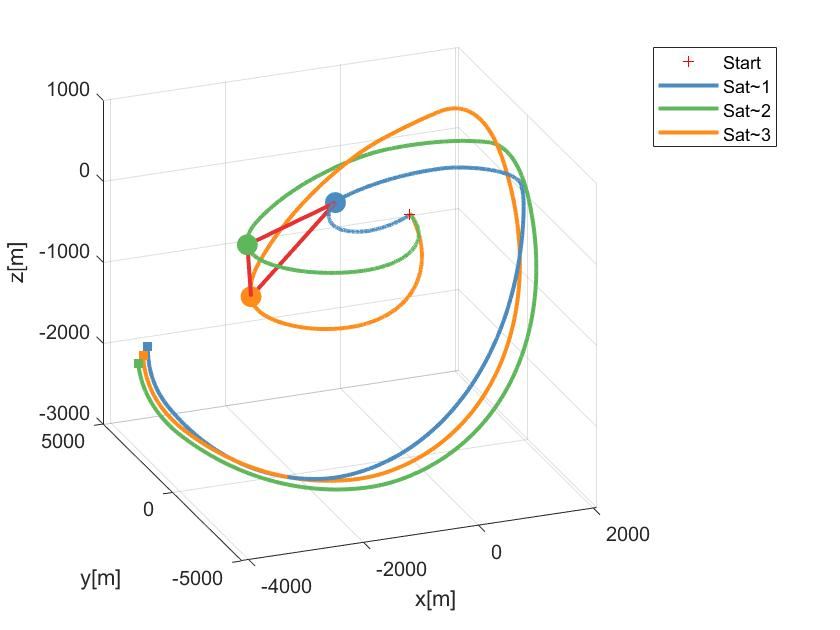
\includegraphics[width=\textwidth]{trajectories-1}
\end{subfigure}

\hfill

\begin{subfigure}{0.4\textwidth}
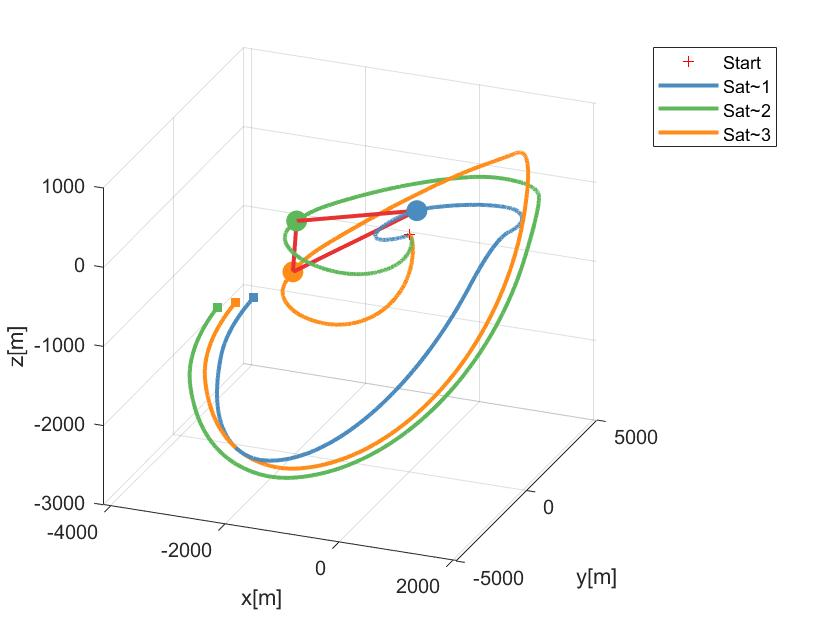
\includegraphics[width=\textwidth]{trajectories-2}
\end{subfigure}

\caption{Satelite Trajectories}
\label{fig:trajectories}
\end{figure}

The actuation forces which allow the satellites to complete these
maneuvers are shown in Figure \ref{fig:orbitals}.

\begin{figure}
\centering

\begin{subfigure}{0.4\textwidth}
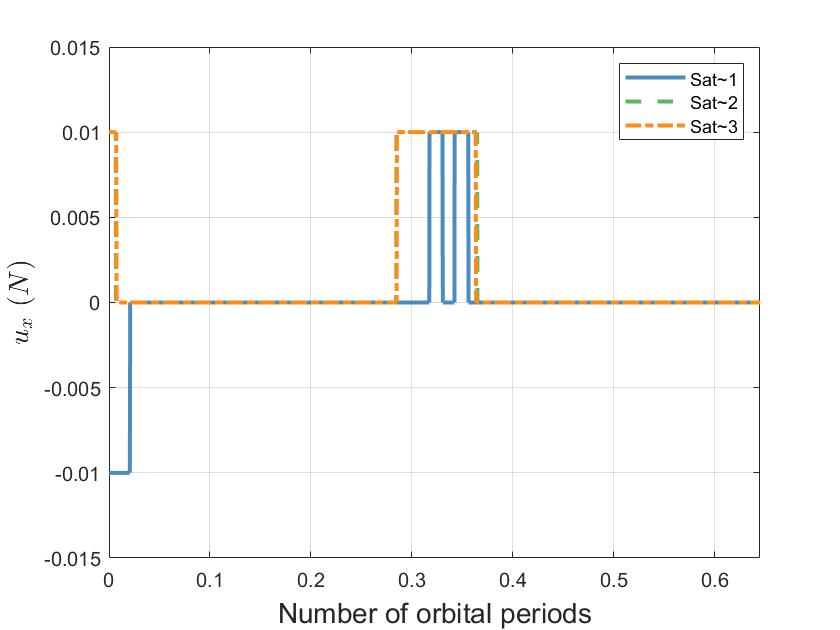
\includegraphics[width=\textwidth]{orbital-periods-1}
\end{subfigure}
\hfill
\begin{subfigure}{0.4\textwidth}
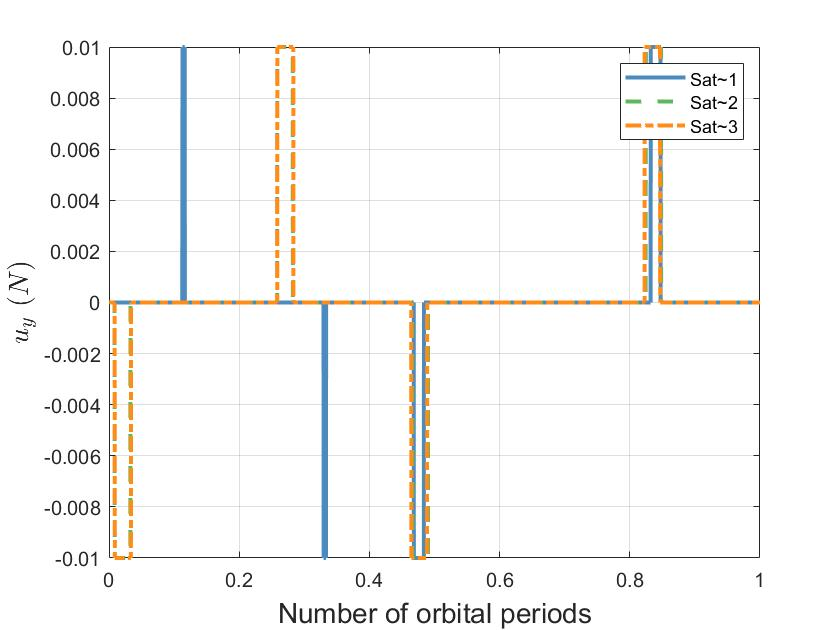
\includegraphics[width=\textwidth]{orbital-periods-2}
\end{subfigure}
\hfill
\begin{subfigure}{0.4\textwidth}
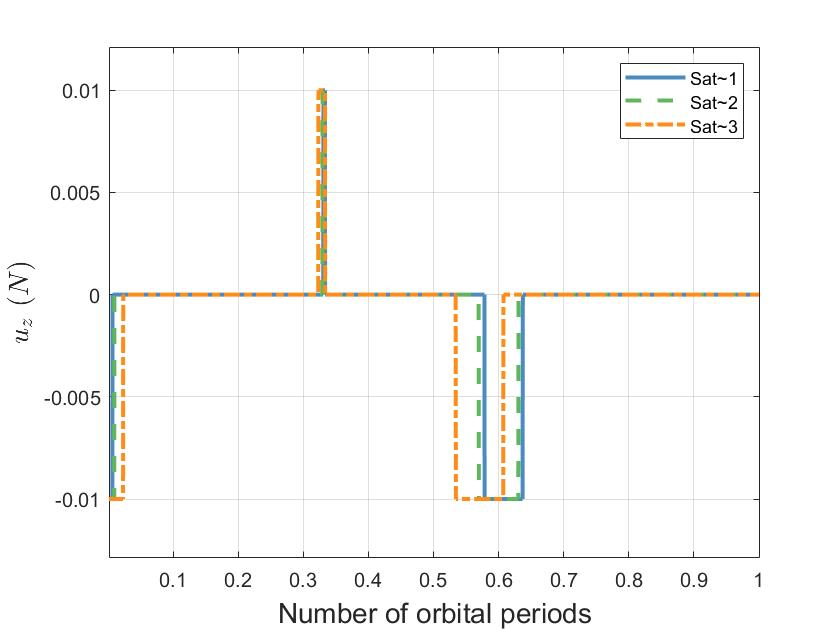
\includegraphics[width=\textwidth]{orbital-periods-3}
\end{subfigure}

\caption{Orbital Periods}
\label{fig:orbitals}
\end{figure}

These actuation profiles can be coupled with magnetorquers to compute
the final thrust vectors for each satellite.

In the following table, we present the absolute impulsive actuations
by each CubeSat in making these maneuvers possible.

\begin{tabular}{|l|l|}
\hline
Index & Absolute Impulsive Actuation $(\int_{0}^{T} (|u_x| + |u_y| + |u_z|) dt)$\\
\hline
Sat-1 & 10.8154 N-s\\
Sat-2 & 17.1647 N-s\\
Sat-3 & 19.0752 N-s\\
\hline
\end{tabular}
\\

Total absolute impulsive actuation by three satellites is
$\sum_{i=1}^{N} \int_{0}^{T} (|u_{xi}(t)| + |u_{yi}(t)| + |u_{zi}(t)|) dt = 47.0553$ N-s.
